\documentclass[pdftex,12pt,a4paper]{report}
\usepackage[portuges]{babel}
\usepackage[utf8]{inputenc}
\usepackage{enumerate}
\usepackage{graphicx}
\usepackage{listings}
\usepackage{verbatim}
\usepackage{indentfirst}
\usepackage{listings, xcolor}
\usepackage{float}
\usepackage{hyperref}
\usepackage{pdfpages}
\usepackage{makecell}
\usepackage{multicol}
\usepackage{blindtext}
\usepackage{adjustbox}
\usepackage{listings}
\usepackage{times}
\usepackage{color}
\graphicspath{{./figs/}}
\definecolor{dkgreen}{rgb}{0,0.6,0}
\definecolor{gray}{rgb}{0.5,0.5,0.5}
\definecolor{mauve}{rgb}{0.58,0,0.82}

\lstset{frame=tb,
  language=Java,
  aboveskip=3mm,
  belowskip=3mm,
  showstringspaces=false,
  columns=flexible,
  basicstyle={\small\ttfamily},
  numbers=none,
  numberstyle=\tiny\color{gray},
  keywordstyle=\color{blue},
  commentstyle=\color{dkgreen},
  stringstyle=\color{mauve},
  breaklines=true,
  breakatwhitespace=true,
  tabsize=3
}


\begin{document}

\newpage
\begin{titlepage}

\newgeometry{left=5cm,top=0cm}

\begin{minipage}{0.6\textwidth}
\begin{flushleft} 

\includegraphics[width=\textwidth]{./Imagens/logo.png}
\end{flushleft}
\end{minipage}

\vspace{3cm}

\Huge
\textbf{SI - Sistemas Autónomos\\}

\huge
\textit{Sistemas Emocionais em}

\textit{Programação de Robots}



\vfill
\normalsize

André Gonçalves, A75625

Miguel Miranda, A74726

Rogério Moreira, A74634

Tiago Sá, A71835

\vfill
Braga, {\today}

\end{titlepage}
\restoregeometry
\newpage

\newpage

\begin{abstract}

O presente trabalho tem como objetivo o desenvolvimento de um Sistema de Partilha de Bicicletas que permita ao utilizador alugar bicicletas para realizar viagens curtas. Pretende-se assim desenvolver um sistema multi-agente utilizando o ambiente de desenvolvimento JADE, complementando com JADEX e JESS.

\end{abstract}

\newpage

\newpage
\section{Introdução}\label{sec:Introduction}

Quase todos os dias ouvimos falar em sistemas de aprendizagem. Tudo é inteligente, seja o frigorífico em nossa casa ou a análise dos nossos exames médicos num hospital. Contudo, nem sempre percebemos os sistemas que estão por detrás dessa inteligência. Torna-se portanto essencial perceber os vários tipos de aprendizagem atualmente existentes. 
Neste trabalho exploramos três áreas: Aprendizagem por Reforço, Redes Neuronais Artificiais e Algoritmos Genéticos.
Para cada um deles são explorados os seguintes tópicos:

\begin{enumerate}
\item Descrição característica;
\item De que modo exibe a capacidade de aprendizagem;
\item Que ferramentas de desenvolvimento existem;
\item Que soluções de mercado existem no mercado baseadas em cada tema.
\end{enumerate}

Numa fase inicial do documento são descritos os dois primeiros pontos para cada área de aprendizagem e numa fase posterior são descritos as ferramentas e as soluções existentes no mercado para cada uma das áreas.
\newpage

\newpage
\section{Trabalho Prático 1}\label{sec:Tp1}

\subsection{Code Smell detetados e respetivo Refactoring}

\textbf{Long Method}

\noindent\begin{minipage}{.45\textwidth}
\begin{lstlisting}[breaklines,caption=Original,frame=tlrb,language=java]{Name}
 public void portfolioUpdater(){
    /*42 linhas*/
    }, 5000,200000);
   }
}
\end{lstlisting}
\end{minipage}\hfill
\begin{minipage}{.45\textwidth}
\begin{lstlisting}[breaklines,caption=Refactored,frame=tlrb,language=java]{Name}
   public void atualizaUsers(){
     allUsers.entrySet().forEach((u) -> {
        it.forEach((c) -> {
        atualizaCFD(c);
       });
    });}
    
 public void portfolioUpdater(){
    atualizaPortfolio();
    }, 5000,200000);
   }
}
\end{lstlisting}
\end{minipage}
\vspace{4mm}
\newline
O refactoring aplicado foi Extract Method, dividiu-se o método original em três métodos distintos. Tornando o método original mais pequeno e portanto, de mais fácil leitura e compreensão.

\vspace{5mm}
\textbf{Large Class}

Verificou-se que as classes Trader continha muitos métodos e linhas de código. Portanto, identificou-se o code smell Large Class. O refactor usado para resolver o problema foi o \textbf{Extract Interface}, ou seja, criou-se uma interface a partir da classe Trader, pertimindo assim uma melhor compreensão da classe.
\newpage

\textbf{Switch Statements}

\noindent\begin{minipage}{.45\textwidth}
\begin{lstlisting}[breaklines,caption=Original,frame=tlrb,language=java]{Name}
updater.start();
do{
menumain.executa();
switch(menumain.getOpcao()){
case 1:
signIn();
break;
case 2:
signUp();
break;
}
}while (menumain.getOpcao()!=0);
\end{lstlisting}
\end{minipage}\hfill
\begin{minipage}{.45\textwidth}
\begin{lstlisting}[breaklines,caption=Refactored,frame=tlrb,language=java]{Name}
public enum MenuInicial {
SIGNIN(1, TraderApp::signIn),
SIGNUP(2, TraderApp::signUp),
UNKNOWN(3, () -> doSomething());
private int value;
 private Runnable execution;
private MenuInicial(int val, Runnable toRun) {
    int value = val;
    execution = toRun;
}
public void execute() { 
    execution.run();
}
static void execute(int code) {
    for (MenuInicial item : values()) {
        if (item.value == code) {
            item.run(); break;
        }
    }
    throw new IAException("unknown");
    }
};
\end{lstlisting}
\end{minipage}

Verificou-se que havia um code smell relacionado com \textbf{Switch Statements}. Para isto cria-se uma classe Enum para cada menu e o utilizador invoca a opção a que corresponde uma função.

\newpage
\textbf{Temporary Field Smell}

\noindent\begin{minipage}{.45\textwidth}
\begin{lstlisting}[breaklines,caption=Original,frame=tlrb,language=java]{Name}
public class Trader implements Serializable{
private boolean logged = false;
private User loggedUser;
private Map<String,User> allUsers = new TreeMap<>();
\end{lstlisting}
\end{minipage}\hfill
\begin{minipage}{.45\textwidth}
\begin{lstlisting}[breaklines,caption=Refactored,frame=tlrb,language=java]{Name}
ppublic class Trader implements Serializable{
private User loggedUser;
private Map<String,User> allUsers = new TreeMap<>();
\end{lstlisting}
\end{minipage}

Na classe Trader era utilizada uma variável de instância "logged" que era apenas usada em alguns casos, não era crucial uma vez que a mesma informação estava disponível noutra variável de instância "loggedUser". Posto isto, foi decidido remover a variável e utilizar apenas a variável "loggedUser". Caso esta esteja a null então é porque não há nenhum utilizado logado, caso contrário há.

\vspace{5mm}
\textbf{Comments}

Documentou-se as maiores classes TraderApp e Trader já que não apresentavam comentários a nenhuma função. Teve-se também em conta a relevância dos comentários em cada função, garantindo que realmente acrescentariam informação.

\subsection{Métricas antes e depois do refactoring}

Para que se possa perceber quais as implicações do refactoring no código foram medidas uma série de itens antes e depois do processo. Existem métricas estáticas (ex: número de linhas de uma classe) e métricas dinâmicas, medidas em tempo de execução (ex: tempo para o utilizador executar x tarefas).
As tarefas para as métricas dinâmicas são as seguintes:
\vspace{5mm}
\newline A \textbf{tarefa 1} consistia na seguinte sequência encadeada de passos:

\begin{enumerate}
    \item Registar utilizador
    \item Login do utilizador
    \item Comprar CFD
    \item Fechar sessão
\end{enumerate}

A \textbf{tarefa 2} consistia na seguinte sequência encadeada de passos:

\begin{enumerate}
    \item Login do utilizador
    \item Vender CFD
    \item Fechar sessão
\end{enumerate}

\newpage

A \textbf{tarefa 3} consistia na seguinte sequência encadeada de passos:

\begin{enumerate}
    \item Registar utilizador
    \item Login do utilizador
    \item Adicionar ativo à watchlist
    \item Imprimir watchlist
    \item Fechar sessão
\end{enumerate}

De seguida listam-se os resultados das medições.
\vspace{5mm}
\newline\textbf{Antes do Refactoring}

\begin{table}[ht]
\centering
\begin{adjustbox}{width=1\textwidth}
\small
\begin{tabular}{|l|l|l|l|l|l|l|l|l|l|l|l|l|}
\hline
Classe                       & Nº de Linhas & Expressões & \% Ramos usados & Chamadas & \% Comentários & Classes & Métodos/Classes & Média de Expressões/Método & Complexidade máxima & Profundidade máxima & Profundidade média & Complexidade média \\ \hline
Trader                       & 188          & 125        & 16.8            & 132      & 5.3            & 2       & 11.50           & 4.30                       & 9                   & 9+                  & 2.99               & 3.04               \\ \hline
TraderApp                    & 252          & 185        & 19.5            & 141      & 3.2            & 2       & 7.50            & 11.13                      & 7                   & 5                   & 2.58               & 2.87               \\ \hline
Menu                         & 60           & 41         & 17.1            & 16       & 1.7            & 1       & 5.00            & 5.60                       & 5                   & 4                   & 1.85               & 2.40               \\ \hline
StockHelper                  & 32           & 19         & 21.1            & 4        & 0.0            & 1       & 3.00            & 4.00                       & 3                   & 3                   & 1.63               & 2.33               \\ \hline
CFD                          & 97           & 55         & 16.4            & 9        & 9.3            & 1       & 9.00            & 3.78                       & 10                  & 3                   & 1.69               & 2.00               \\ \hline
StockFetcher                 & 85           & 61         & 1.6             & 32       & 32.9           & 1       & 1.00            & 50.00                      & 2                   & 3                   & 2.11               & 2.00               \\ \hline
User                         & 123          & 71         & 8.5             & 28       & 0.0            & 1       & 16.00           & 2.75                       & 7                   & 3                   & 1.63               & 1.38               \\ \hline
CompanyNotFoundException     & 16           & 4          & 0               & 1        & 56.3           & 1       & 1.00            & 1.00                       & 1                   & 2                   & 0.75               & 1.00               \\ \hline
ComparatorUser               & 10           & 5          & 0               & 1        & 0.0            & 1       & 1.00            & 1.00                       & 1                   & 2                   & 0.60               & 1.00               \\ \hline
SaldoException               & 16           & 4          & 0               & 1        & 56.3           & 1       & 1.00            & 1.00                       & 1                   & 2                   & 0.75               & 1.00               \\ \hline
SemAutorizacaoException      & 16           & 4          & 0               & 1        & 56.3           & 1       & 1.00            & 1.00                       & 1                   & 2                   & 0.75               & 1.00               \\ \hline
SerializationUtil            & 31           & 22         & 0               & 10       & 0.0            & 1       & 2.00            & 5.50                       & 1                   & 2                   & 1.09               & 1.00               \\ \hline
Stock                        & 125          & 80         & 0               & 0        & 0.0            & 1       & 20.00           & 1.90                       & 1                   & 2                   & 1.44               & 1.00               \\ \hline
UtilizadorExistenteException & 16           & 4          & 0               & 1        & 56.3           & 1       & 1.00            & 1.00                       & 1                   & 2                   & 0.75               & 1.00               \\ \hline
Utils                        & 25           & 4          & 0               & 1        & 36.0           & 1       & 1.00            & 1.00                       & 1                   & 2                   & 0.75               & 1.00               \\ \hline
CFDtype                      & 16           & 3          & 0               & 0        & 60.0           & 1       & 0.00            & 0.00                       & 0                   & 1                   & 0.33               & 0.00               \\ \hline
\end{tabular}
\end{adjustbox}
\caption{Métricas estáticas das classes}
\end{table}

\begin{table}[]
\centering
\begin{tabular}{|l|l|l|}
\hline
Tarefa   & Elapsed Time & CPU Time    \\ \hline
Tarefa 1 & 0.454875s    & 28.6271518s \\ \hline
Tarefa 2 & 0.334007s    & 65.1614337s \\ \hline
Tarefa 3 & 0.448339s    & 22.2790403s \\ \hline
\end{tabular}
\caption{Métricas dinâmicas das classes}
\end{table}

\newpage

\textbf{Depois do Refactoring}

\begin{table}[ht]
\centering
\begin{adjustbox}{width=1\textwidth}
\small
\begin{tabular}{|l|l|l|l|l|l|l|l|l|l|l|l|l|}
\hline
Classe                       & Nº de Linhas & Expressões & \% Ramos usados & Chamadas & \% Comentários & Classes & Métodos/Classes & Média de Expressões/Método & Complexidade máxima & Profundidade máxima & Profundidade média & Complexidade média \\ \hline
CFD                          & 97           & 55         & 16.4            & 9        & 9.3            & 1       & 9.00            & 3.78                       & 10                  & 3                   & 1.69               & 2.00               \\ \hline
CFDtype                      & 15           & 3          & 0.0             & 0        & 60.0           & 1       & 0.00            & 0.00                       & 0                   & 1                   & 0.33               & 0.00               \\ \hline
CompanyNotFoundException     & 16           & 4          & 0.0             & 1        & 56.3           & 1       & 1.00            & 1.00                       & 1                   & 2                   & 0.75               & 1.00               \\ \hline
ComparatorUser               & 10           & 5          & 0.0             & 1        & 0.0            & 1       & 1.00            & 1.00                       & 1                   & 2                   & 0.60               & 1.00               \\ \hline
Menu                         & 60           & 41         & 17.1            & 16       & 1.7            & 1       & 5.00            & 5.60                       & 5                   & 4                   & 1.85               & 2.40               \\ \hline
MenuInicial                  & 28           & 16         & 12.5            & 6        & 0.0            & 1       & 3.00            & 2.33                       & 3                   & 4                   & 1.44               & 1.67               \\ \hline
SaldoException               & 16           & 4          & 0.0             & 1        & 56.3           & 1       & 1.00            & 1.00                       & 1                   & 2                   & 0.75               & 1.00               \\ \hline
SemAutorizacaoException      & 16           & 4          & 0.0             & 1        & 56.3           & 1       & 1.00            & 1.00                       & 1                   & 2                   & 0.75               & 1.00               \\ \hline
SerializationUtil            & 31           & 22         & 0.0             & 10       & 0.0            & 1       & 2.00            & 5.50                       & 1                   & 2                   & 1.09               & 1.00               \\ \hline
Stock                        & 125          & 80         & 0.0             & 0        & 0.0            & 1       & 20.00           & 1.90                       & 1                   & 2                   & 1.44               & 1.00               \\ \hline
StockFetcher                 & 85           & 61         & 1.6             & 32       & 32.9           & 1       & 1.00            & 50.00                      & 2                   & 3                   & 2.11               & 2.00               \\ \hline
StockHelper                  & 32           & 19         & 21.1            & 4        & 0.0            & 1       & 3.00            & 4.00                       & 3                   & 3                   & 1.63               & 2.33               \\ \hline
Trader                       & 192          & 119        & 17.6            & 131      & 0.0            & 2       & 11.00           & 4.32                       & 9                   & 9+                  & 3.05               & 3.14               \\ \hline
TraderApp                    & 285          & 185        & 19.5            & 141      & 14.4           & 2       & 7.50            & 11.13                      & 7                   & 5                   & 2.58               & 2.87               \\ \hline
TraderInterface              & 40           & 20         & 0.0             & 0        & 0.0            & 1       & 16.00           & 0.00                       & 0                   & 1                   & 0.80               & 0.00               \\ \hline
User                         & 123          & 71         & 8.5             & 28       & 0.0            & 1       & 16.00           & 2.75                       & 7                   & 3                   & 1.63               & 1.38               \\ \hline
UtilizadorExistenteException & 16           & 4          & 0.0             & 1        & 56.3           & 1       & 1.00            & 1.00                       & 1                   & 2                   & 0.75               & 0.00               \\ \hline
Utils                        & 25           & 4          & 0.0             & 1        & 36.0           & 1       & 1.00            & 1.00                       & 1                   & 2                   & 0.75               & 0.00               \\ \hline
\end{tabular}
\end{adjustbox}
\caption{Métricas estáticas das classes}
\end{table}

\begin{table}[]
\centering
\begin{tabular}{|l|l|l|}
\hline
Tarefa   & Elapsed Time & CPU Time    \\ \hline
Tarefa 1 & 0.335594s    & 16.8276316s \\ \hline
Tarefa 2 & 0.246420s    & 38.3032377s \\ \hline
Tarefa 3 & 0.330771s    & 13.0960804s \\ \hline
\end{tabular}
\caption{Métricas dinâmicas das classes}
\end{table}

\newpage

\newpage
\section*{Parte 2}\label{sec:parte2}
\subsection*{Criação do Schema}

Uma vez recolhidos os dados, foi necessário guardar os mesmos de forma organizada em estruturas independentes daquelas já existentes na base de dados Oracle. Para tal procedemos à criação do tablespace, datafile e utilizador que permitiram que tal aconteça.

\subsection*{Tablespace e Datafile}
 
Antes de ser feito o armazenamento de dados na base de dados, foi criado em primeiro lugar um \textit{tablespace} permanente, \textbf{assignment\_tables}, que conterá todos os objetos do utilizador  da nossa BD, armazenados fisicamente no \textit{datafile} \textbf{assignment\_tables\_1}:

\begin{verbatim}
CREATE TABLESPACE assignment_tables
    DATAFILE '\u01\app\oracle\oradata\orcl12\orcl\assignment_tables_1.dbf'
        SIZE 200M;
\end{verbatim}
  
Em seguida, foi criado o \textit{tablespace} temporário, onde são armazenados os dados temporários de uma determinada sessão por um determinado período de tempo. Este \textit{tablespace} possui um \textit{tempfile} e, não um \textit{datafile}, e é utilizado quando um utilizador, ao qual o tablespace temporário foi atribuído, inicia operações. Sendo assim, o tablespace temporário armazena os dados temporários utilizados em transações de utilizadores:

\begin{verbatim}
CREATE TEMPORARY TABLESPACE assignment_temp
    TEMPFILE '\u01\app\oracle\oradata\orcl12\orcl\assignment_temp_1.dbf'
        SIZE 50M
        AUTOEXTEND ON;
\end{verbatim}

\subsection*{User e Grants}

Uma vez criados os \textit{tablespaces} e \textit{datafiles}, foi criada a conta do utilizador através da qual é feito o login à base de dados. Para criar o utilizador foi especificado que os objetos por ele criados ficariam armazenados no \textit{tablespace}  referido anteriormente:

\begin{verbatim}
CREATE USER mic
    IDENTIFIED BY oracle
    DEFAULT TABLESPACE assignment_tables
    TEMPORARY TABLESPACE assignment_temp;

\end{verbatim}


O privilégio CREATE SESSION garante que o utilizador criado se consiga conectar à base de dados, e com os restantes privilégios concedidos este pode criar e manipular os objetos da BD:

\begin{verbatim}
GRANT CREATE SESSION TO mic;
GRANT CREATE TABLE TO mic;
GRANT CREATE VIEW TO mic;
GRANT CREATE ANY TRIGGER TO mic;
GRANT CREATE ANY PROCEDURE TO mic;
GRANT CREATE SEQUENCE TO mic;
GRANT CREATE SYNONYM TO mic;
\end{verbatim}

Por defeito, ao ser criado o utilizador não tem quota no tablespace, sendo necessária a sua atribuição para que este possa criar objetos:
\begin{verbatim}
ALTER USER mic QUOTA 200M ON assignment_tables;
\end{verbatim}

Depois de ser estabelecida uma ligação à base de dados com este utilizador, foram criadas as tabelas e procedimentos necessários para armazenar de forma correta os dados, como veremos na secção seguinte.

\subsection*{Tabelas}
De forma a poder guardar os dados inicialmente recolhidos, foi necessária a criação de tabelas para esse efeito. Tendo em conta que para a monitorização da base de dados seria necessário atualizar  constantemente os dados recolhidos e guardar toda a informação que a cada momento é consultada, para algumas das tabelas criadas foi também gerada uma tabela de "histórico", isto é, uma tabela que para uma determinada instância de dados vai guardar as mudanças relativas a esses dados. Para permitir registar estas mudanças, foi necessário associar aos dados recolhidos um \textit{timestamp}. Mais à frente são explicadas com mais detalhe as tabelas de histórico

Em seguida é apresentada para cada tabela a DDL para a sua geração, bem como uma breve explicação dos atributos e chaves que compõe a tabela.
\subsubsection*{Tablespaces}

A tabela \textbf{tablespaces} armazena todos os dados recolhidos considerados relevantes em relação aos \textit{tablespaces} da base de dados Oracle, o que incluí o seu nome, o espaço utilizado, o espaço livre, o espaço total e a percentagem de espaço utilizado.

A chave primária desta tabela é o nome do tablespace visto ser o único atributo que identifica univocamente uma instância da entidade:

\begin{verbatim}
CREATE TABLE tablespaces
    (   tablespace_name varchar2(50) not null,
        used_MB number not null,
        free_MB number not null,
        total_MB number not null,
        percentage_used number not null,
        timestamp timestamp not null,
        CONSTRAINT tablespaces_pk PRIMARY KEY (tablespace_name)
    );
    

\end{verbatim}
\subsubsection*{Datafiles}

A tabela \textbf{datafiles} armazena, tal como o nome indica, os dados recolhidos relativamente aos \textit{datafiles} do sistema. Estes são o identificador do datafile (file\_id), o nome do datafile, o nome do tablespace a que este está associado, o seu tamanho totalm o tamanho utilizado, o tamanho livre, e a percentagem de tamanho utilizado.

A chave primária desta tabela é o file\_id do datafile, por ser o atributo de menor tamanho e o único que identfica unicamente uma instância desta tabela.

 A tabela \textbf{datafiles} tem uma chave estrangeira, tablespace\_name, que faz referência à chave primária da tabela \textbf{tablespaces}. Cada \textit{tablespace} numa base de dados Oracle consiste em um ou mais \textit{datafiles}, o que justifica a existência deste relacionamento:



\begin{verbatim}
CREATE TABLE datafiles
    (   file_id number not null,
        datafile_name varchar2(512) not null,
        tablespace_name varchar2(50) not null,
        total_MB number not null,
        used_MB number not null,
        free_MB number not null,
        percentage_used number not null,
        timestamp timestamp not null,
        CONSTRAINT datafiles_pk PRIMARY KEY(file_id),
        CONSTRAINT fk_tablespaces FOREIGN KEY(tablespace_name)
            REFERENCES tablespaces(tablespace_name)
    );
\end{verbatim}
\subsubsection*{Users}

Na tabela \textbf{users} são armazenados os dados recolhidos relativamente aos utilizadores da base de dados Oracle, nomeadamente o user identificador, o nome, o tablespace permanente a que estão associados, assim como o temporário, o estado da conta do utilizador, a quota no tablespace, os privilégios que lhe foram concedidos e a sua utiliação de cpu.

A chave primária de \textbf{users} é o user\_id, por ser o único atributo que identifica univocamente um utilizador.

Esta tabela tem uma chave estrangeira, default\_tablespaces, que faz referência à chave primária da tabela \textbf{tablespaces}, ou seja ao nome do tablespace:
\begin{verbatim}

CREATE TABLE users
    (   user_id number not null,
        name varchar2(50) not null,
        default_tablespace varchar2(50) not null,
        temporary_tablespace varchar2(50) not null,
        account_status varchar2(20) not null,
        quota number not null,
        privilege varchar2(50),
        cpu_usage number,
        timestamp timestamp not null,
        CONSTRAINT users_pk PRIMARY KEY(user_id),
        CONSTRAINT fk_tablespaces_users FOREIGN KEY(default_tablespace)
            REFERENCES tablespaces(tablespace_name)
    );
\end{verbatim}
\subsubsection*{Tables}

Nesta tabela armazenam-se todas as informações relativas às tabelas da base de dados, nomeadamente o nome do dono (utilizador) da tabela, o id desse utilizador, o nome da tabela, o nome do \textit{tablespace} onde a tabela foi criada, o número de acessos à tabela e o número de registos da mesma.

A chave primária desta de \textbf{tables} é composta pelo nome da tabela e o identificador do utilizador que a criou, uma vez que esta á única forma de identificar unicamente uma instância de \textbf{tables}. Diferentes utilizadores podem ter tabelas com o mesmo nome, e daí o nome da tabela não ser suficiente para constituir a chave primária. Desta composição justifica-se a existência da chave estrangeira owner\_id, que faz referência à chave primária da tabela \textbf{users}, ou seja o identificador do utiizador.



\begin{verbatim}
CREATE TABLE tables
    (   owner_name varchar2(30) not null,
        owner_id number not null,
        name varchar2(30) not null,
        correspondent_tablespace varchar2(50),
        nr_of_accesses number not null,
        nr_of_regists number not null,
        dropped varchar2(20) not null,
        timestamp timestamp not null,
        CONSTRAINT tables_pk PRIMARY KEY(owner_id,name),
        CONSTRAINT fk_users_tables FOREIGN KEY(owner_id)
            REFERENCES users(user_id)        
    );
\end{verbatim}
\subsubsection*{Memory}

Os dados recolhidos relativamente à memória do sistema são guardados na tabela \textbf{memory}, e consistem na memória utilizada, na memória livre e na percentagem de memória livre.

A chave primária desta tabela é o timestamp, que a cada momento da recolha de informação permite identificar univocamente o estado da memória:
\begin{verbatim}
CREATE TABLE memory
    (   total_size_bytes number not null,
        free_size_bytes number not null,
        percentage_free number not null,
        timestamp timestamp not null,
        CONSTRAINT memory_pk PRIMARY KEY (timestamp)
    );
\end{verbatim}
\subsubsection*{Sessions}

Os dados referentes às sessões na base de dados encontram-se armazenados na tabela \textbf{sessions}. É guardada informação relativamente ao id da sessão, ao nome do utilizador associado à sessão, o id associado a esse utilizador, o nome do \textit{schema} da sessão, e há quanto tempo a sessão foi iniciada.

A chave primária desta tabela é composta pelo id da sessão (session\_id) e o timestamp em que a informação sobre as sessões foi recolhida.

\textbf{Sessions} tem uma chave estrangeira, \textbf{user\_id}, que faz referência à chave primária da tabela \textbf{users}, isto é ao id do utilizador, uma vez que um utilizador pode ter uma ou mais sessões ativas.

\begin{verbatim}
CREATE TABLE sessions
    (   session_id number not null,
        username varchar2(50) not null,
        user_id number not null,
        schema_name varchar2(50) not null,
        login_time varchar2(50) not null,
        timestamp timestamp not null,
        CONSTRAINT sessions_pk PRIMARY KEY (session_id,timestamp),
        CONSTRAINT fk_users FOREIGN KEY (user_id)
            REFERENCES users(user_id)
        
    );
\end{verbatim}
\subsubsection*{Io\_reads}

A tabela \textbf{io\_reads} armazena a informação relativa às leituras ao disco, que consiste no nome da métrica, o tempo de início da leitura, o tempo final da leitura e o valor da métrica.

A chave primária de \textbf{io\_reads} é o timestamp visto ser o único atributo que identifica univocamente uma instância desta tabela.
\begin{verbatim}
    
CREATE TABLE io_reads
    (
    metric_name varchar2(64) not null,
    begin_time timestamp not null,
    end_time timestamp not null,
    value number not null,
    timestamp timestamp not null,
    CONSTRAINT io_reads_pk PRIMARY KEY (timestamp)
    );
\end{verbatim}
\subsubsection*{Io\_writes}
A tabela \textbf{io\_writes} armazena a informação relativa às escritas ao disco, que consiste no nome da métrica, o tempo de início da leitura, o tempo final da leitura e o valor da métrica.

A chave primária de \textbf{io\_writes} é o timestamp, que tal como para a tabela \textbf{io\_reads}, é o único atributo que identifica univocamente uma instância desta tabela.
\begin{verbatim}
CREATE TABLE io_writes
    (
    metric_name varchar2(64) not null,
    begin_time timestamp not null,
    end_time timestamp not null,
    value number not null,
    timestamp timestamp not null,
    CONSTRAINT io_writes_pk PRIMARY KEY (timestamp)
    );
    
\end{verbatim}
\subsection*{Histórico e Triggers}
Como referido anteriormente, para algumas das tabelas foi necessário criar uma tabela de histórico para guardar registo das mudanças aos dados, de cada vez que são atualizados. A tabela de histórico é também útil para manter as tabelas "ativas" na base de dados, ou seja com a informação mais recente, com um tamanho consideravelmente reduzido. As tabelas \textbf{tablespaces}, \textbf{datafiles}, \textbf{users}, \textbf{tables} e \textbf{sessions} têm uma tabela de histórico associada, cuja única diferença em relação à tabela "mãe" é a de a chave primária ser composta também pelo timestamp.

Para guardar as mudanças  foi criado um\textit{trigger} que é acionado sempre que há atualização dos dados na tabela a que a tabela de histórico se refere. A título de exemplo, é mostrada a tabela de histórico e trigger para inserção da dados na tabela \textbf{tablespaceshistory}, que se refere aos dados da tabela \textbf{tablespaces}:
\\


\begin{verbatim}
CREATE TABLE tablespaceshistory
    (   tablespace_name varchar2(50) not null,
        used_MB number not null,
        free_MB number not null,
        total_MB number not null,
        percentage_used number not null,
        timestamp timestamp not null,
        CONSTRAINT tablespaceshistory_pk PRIMARY KEY (tablespace_name,timestamp)

\end{verbatim}
O \textit{trigger} é do tipo AFTER INSERT, e quando é feita um \textit{update} na tabela \textbf{tablespaces}, pega nos valores que estavam na tabela e insere-os na tabela de histórico:
\begin{verbatim}
CREATE OR REPLACE TRIGGER insert_into_tablespaceshistory
AFTER UPDATE ON tablespaces FOR EACH ROW
BEGIN
    INSERT INTO tablespaceshistory
        (tablespace_name,used_MB,free_MB,total_MB,percentage_used,timestamp)
    VALUES
        (:OLD.tablespace_name,:OLD.used_MB,:OLD.free_MB,:OLD.total_MB,:OLD.percentage_used,:OLD.timestamp);   
END insert_into_tablespaceshistory;
/
\end{verbatim}





\newpage
\subsection*{Modelo Relacional}

\begin{figure}[h!]
 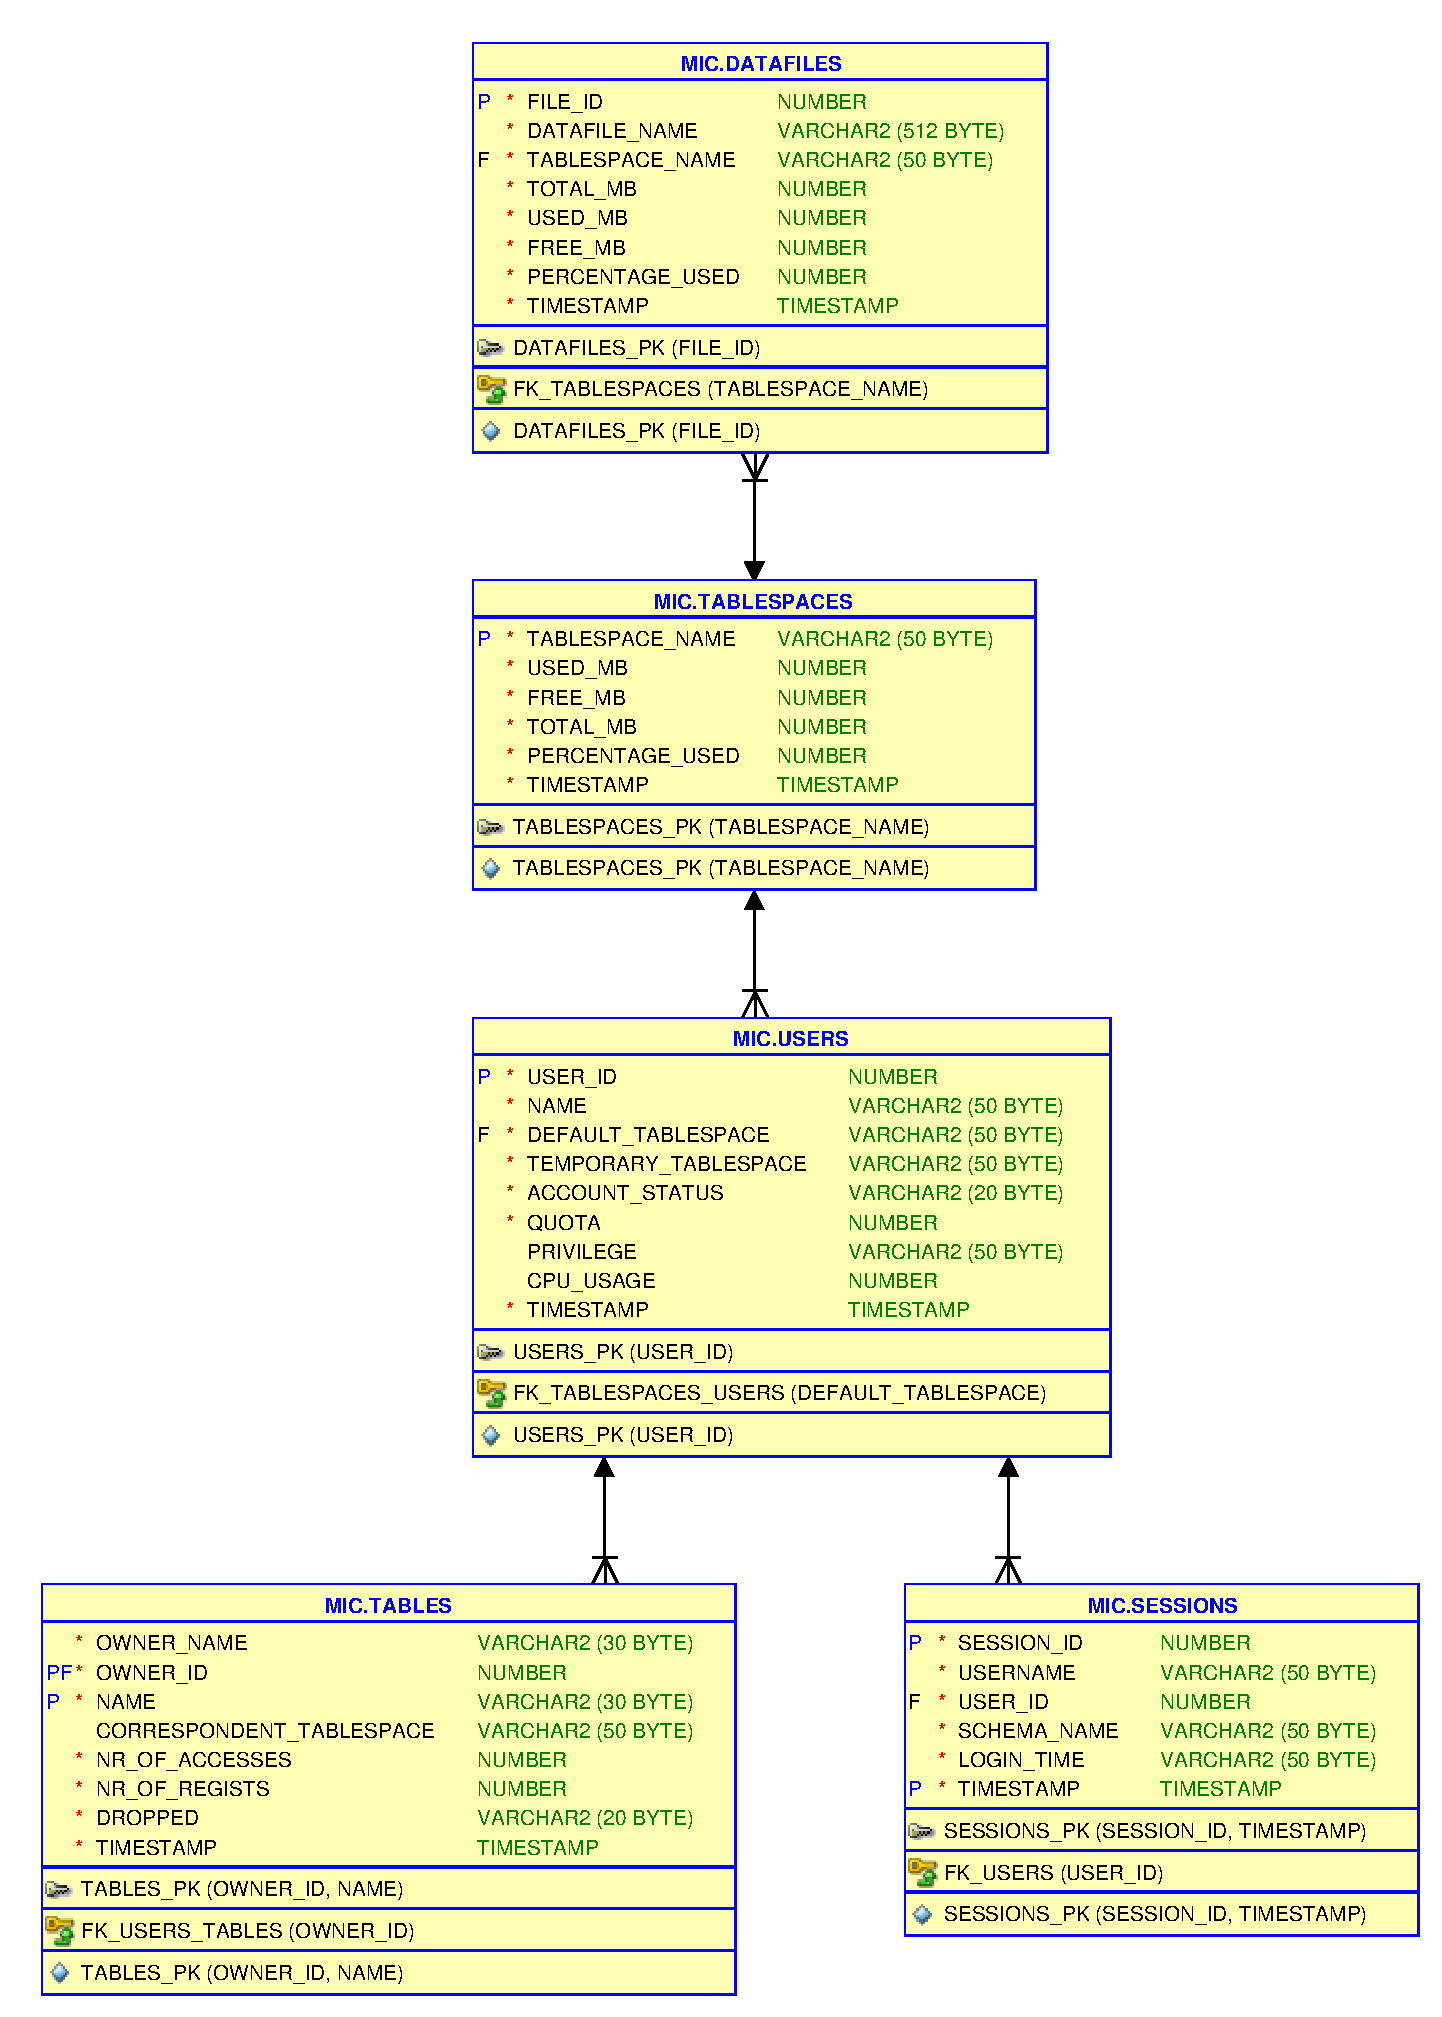
\includegraphics[scale=0.5]{tex/img/modelo_concetual.pdf}
    \caption{Modelo relacional da base de dados.} 
    \label{fig:modelo}
\end{figure}



\newpage

\newpage
\section{Anti-Padrão}\label{sec:ap}

Um dos objetivos iniciais do projeto era a implementação de um anti-padrão, à escolha. O anti-padrão selecionado foi o \textbf{Input Kludge}, que consiste na má gestão dos inputs dos utilizados na interface, ou seja, quando por exemplo o input permite texto livre do utilizador que pode conter texto inválido e prejudicial ao programa.
\newline Para a implementação do anti-padrão foram removidas todas as verificações de texto do input do utilizador. Por exemplo, foram removidas as verificações se a empresa inserida existe, se o email é válido e se o texto é numérico (nos casos em que tem que ser).
\newpage

\subsection{Métricas}

\textbf{Antes da implementação do Anti-Padrão}

\begin{table}[ht]
\centering
\begin{adjustbox}{width=1\textwidth}
\small
\begin{tabular}{|l|l|l|l|l|l|l|l|l|l|l|l|l|}
\hline
Classe                       & Nº de Linhas & Expressões & \% Ramos usados & Chamadas & \% Comentários & Classes & Métodos/Classes & Média de Expressões/Método & Complexidade máxima & Profundidade máxima & Profundidade média & Complexidade média \\ \hline
Asset                        & 57           & 32         & 0.0             & 0        & 0.0            & 1       & 10.00           & 1.60                       & 1                   & 2                   & 1.44               & 1.00               \\ \hline
CFD                          & 102          & 65         & 13.8            & 10       & 0.0            & 1       & 11.00           & 3.82                       & 10                  & 3                   & 1.71               & 1.82               \\ \hline
CFDtype                      & 8            & 3          & 0.0             & 0        & 0.0            & 1       & 0.00            & 0.00                       & 0                   & 1                   & 0.33               & 0.00               \\ \hline
CompanyNotFoundException     & 7            & 4          & 0.0             & 1        & 1.7            & 1       & 1.00            & 1.00                       & 1                   & 2                   & 0.75               & 1.00               \\ \hline
ComparatorUser               & 10           & 5          & 0.0             & 1        & 0.0            & 1       & 1.00            & 1.00                       & 1                   & 2                   & 0.60               & 1.00               \\ \hline
Menu                         & 60           & 41         & 17.1            & 16       & 0.0            & 1       & 5.00            & 5.60                       & 5                   & 4                   & 1.85               & 2.40               \\ \hline
notificationsDAO             & 83           & 60         & 1.7             & 59       & 0.0            & 1       & 4.00            & 11.50                      & 2                   & 3                   & 1.72               & 1.25               \\ \hline
SaldoException               & 7            & 4          & 0.0             & 1        & 0.0            & 1       & 1.00            & 1.00                       & 1                   & 2                   & 0.75               & 1.00               \\ \hline
SemAutorizacaoException      & 7            & 4          & 0.0             & 1        & 0.0            & 1       & 1.00            & 1.00                       & 1                   & 2                   & 0.75               & 1.00               \\ \hline
Trader                       & 217          & 152        & 13.8            & 140      & 0.0            & 3       & 9.00            & 4.52                       & 10                  & 9+                  & 3.32               & 3.00               \\ \hline
TraderApp                    & 284          & 222        & 18.0            & 181      & 0.0            & 3       & 6.00            & 10.94                      & 7                   & 5                   & 2.49               & 2.88               \\ \hline
User                         & 123          & 71         & 8.5             & 28       & 0.0            & 1       & 16.00           & 2.75                       & 7                   & 3                   & 1.63               & 1.38               \\ \hline
userDAO                      & 247          & 173        & 5.2             & 184      & 0.0            & 1       & 12.00           & 12.67                      & 6                   & 5                   & 2.23               & 1.82               \\ \hline
UtilizadorExistenteException & 8            & 4          & 0.0             & 1        & 0.0            & 1       & 1.00            & 1.00                       & 1                   & 2                   & 0.75               & 1.00               \\ \hline
Utils                        & 17           & 4          & 0.0             & 1        & 0.0            & 1       & 1.00            & 1.00                       & 1                   & 2                   & 0.75               & 1.00               \\ \hline
\end{tabular}
\end{adjustbox}
\caption{Métricas estáticas das classes}
\end{table}

\begin{table}[]
\centering
\begin{tabular}{|l|l|l|}
\hline
Tarefa   & Elapsed Time & CPU Time    \\ \hline
Tarefa 1 & 1.423028s    & 38.1617271s \\ \hline
Tarefa 2 & 1.1273s    & 22.0295465s \\ \hline
Tarefa 3 & 1.392363s    & 32.893317s \\ \hline
\end{tabular}
\caption{Métricas dinâmicas das classes}
\end{table}
\newpage
\textbf{Depois da implementação do Anti-Padrão}

\begin{table}[ht]
\centering
\begin{adjustbox}{width=1\textwidth}
\small
\begin{tabular}{|l|l|l|l|l|l|l|l|l|l|l|l|l|}
\hline
Classe                       & Nº de Linhas & Expressões & \% Ramos usados & Chamadas & \% Comentários & Classes & Métodos/Classes & Média de Expressões/Método & Complexidade máxima & Profundidade máxima & Profundidade média & Complexidade média \\ \hline
Asset                        & 57           & 32         & 0.0             & 0        & 0.0            & 1       & 10.00           & 1.60                       & 1                   & 2                   & 1.44               & 1.00               \\ \hline
CFD                          & 102          & 65         & 13.8            & 10       & 0.0            & 1       & 11.00           & 3.82                       & 10                  & 3                   & 1.71               & 1.82               \\ \hline
CFDtype                      & 8            & 3          & 0.0             & 0        & 0.0            & 1       & 0.00            & 0.00                       & 0                   & 1                   & 0.33               & 0.00               \\ \hline
CompanyNotFoundException     & 7            & 4          & 0.0             & 1        & 1.7            & 1       & 1.00            & 1.00                       & 1                   & 2                   & 0.75               & 1.00               \\ \hline
ComparatorUser               & 10           & 5          & 0.0             & 1        & 0.0            & 1       & 1.00            & 1.00                       & 1                   & 2                   & 0.60               & 1.00               \\ \hline
Menu                         & 60           & 41         & 17.1            & 16       & 0.0            & 1       & 5.00            & 5.60                       & 5                   & 4                   & 1.85               & 2.40               \\ \hline
MenuInicial                  & 30           & 17         & 11.8            & 6        & 0.0            & 1       & 3.00            & 2.33                       & 3                   & 4                   & 1.35               & 1.67               \\ \hline
MongoConnection              & 22           & 14         & 0.0             & 4        & 0.0            & 1       & 2.00            & 1.00                       & 1                   & 2                   & 0.71               & 1.00               \\ \hline
notificationsDAO             & 66           & 42         & 2.4             & 45       & 20.9           & 1       & 4.00            & 7.50                       & 2                   & 3                   & 1.71               & 1.25               \\ \hline
SaldoException               & 7            & 4          & 0.0             & 1        & 13.9           & 1       & 1.00            & 1.00                       & 1                   & 2                   & 0.75               & 1.00               \\ \hline
SemAutorizacaoException      & 7            & 4          & 0.0             & 1        & 17.6           & 1       & 1.00            & 1.00                       & 1                   & 2                   & 0.75               & 1.00               \\ \hline
Trader                       & 203          & 144        & 11.1            & 130      & 0.0            & 3       & 9.00            & 4.22                       & 10                  & 9+                  & 3.35               & 3.35               \\ \hline
TraderApp                    & 330          & 229        & 17.2            & 186      & 0.0            & 3       & 6.00            & 11.28                      & 7                   & 5                   & 2.45               & 2.88               \\ \hline
TraderInterface              & 51           & 21         & 0.0             & 0        & 0.0            & 1       & 17.00           & 0.00                       & 0                   & 1                   & 0.81               & 0.00               \\ \hline
User                         & 123          & 71         & 8.5             & 28       & 0.0            & 1       & 16.00           & 2.75                       & 7                   & 3                   & 1.63               & 1.38               \\ \hline
userDAO                      & 203          & 135        & 6.7             & 150      & 0.0            & 1       & 12.00           & 9.67                       & 6                   & 5                   & 2.23               & 1.82               \\ \hline
UtilizadorExistenteException & 8            & 4          & 0.0             & 1        & 0.0            & 1       & 1.00            & 1.00                       & 1                   & 2                   & 0.75               & 1.00               \\ \hline
Utils                        & 17           & 4          & 0.0             & 1        & 0.0            & 1       & 1.00            & 1.00                       & 1                   & 2                   & 0.75               & 1.00               \\ \hline
\end{tabular}
\end{adjustbox}
\caption{Métricas estáticas das classes}
\end{table}

\begin{table}[H]
\centering
\begin{tabular}{|l|l|l|}
\hline
Tarefa   & Elapsed Time & CPU Time    \\ \hline
Tarefa 1 & 0.481010s    & 24.7417182s \\ \hline
Tarefa 2 & 0.381150s    & 14.28260403s \\ \hline
Tarefa 3 & 0.470809s    & 21.3260026s \\ \hline
\end{tabular}
\caption{Métricas dinâmicas das classes}
\end{table}
\newpage

\newpage
\chapter*{Aplicação Web}

A primeira decisão a tomar sobre a construção da aplicação web foi em que linguagem o fazer. Depois de analisar algumas hipóteses, escolhemos desenvolver com \textbf{\href{https://angularjs.org/}{AngularJS}}.
\newline Foram necessários um conjunto de passos iniciais para preparar o ambiente para o desenvolvimento:

\begin{enumerate}
    \item npm install http-server -g
    \item http-server -o
\end{enumerate}

E também preparar a estrutura do projeto:

\begin{itemize}
    \item Criar o ficheiro index.html;
    \item Criar a pasta pages e todas as páginas necessárias ao projeto;
    \item Criar o ficheiro app.js, onde se encontra toda a lógica do programa.
\end{itemize}

Posto isto, foi criada uma página para cada tabela da base de dados correspondente e feito o routing no AngularJS. Em cada uma das páginas existe um controller onde é feito o \$http.GET da API da base de dados. Os dados são tratados e visualizados na página html correspondente.
\newline Para a construção de gráficos foi usada a ferramenta \textbf{\href{https://plot.ly/javascript/}{plotlyJS}}.

\begin{figure}[h!]
 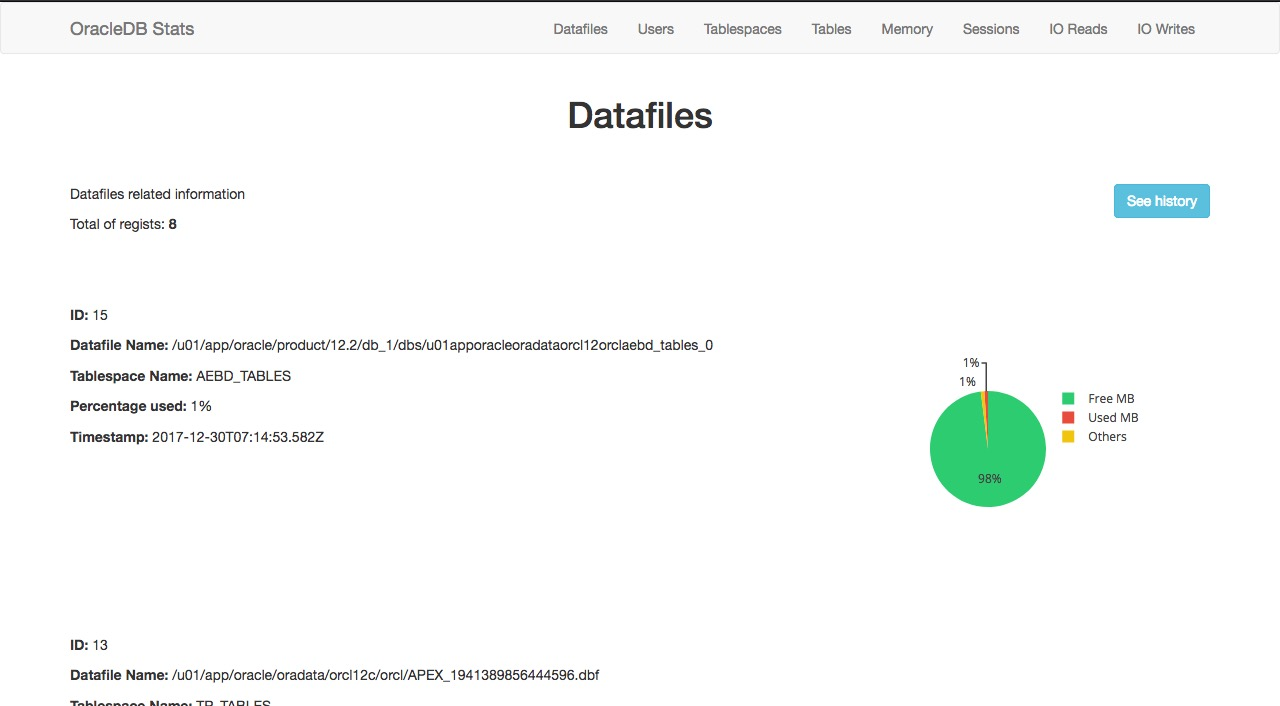
\includegraphics[width=\linewidth]{tex/img/home.jpg}
    \caption{Página correspondente aos Datafiles} 
\end{figure}

\begin{figure}[h!]
 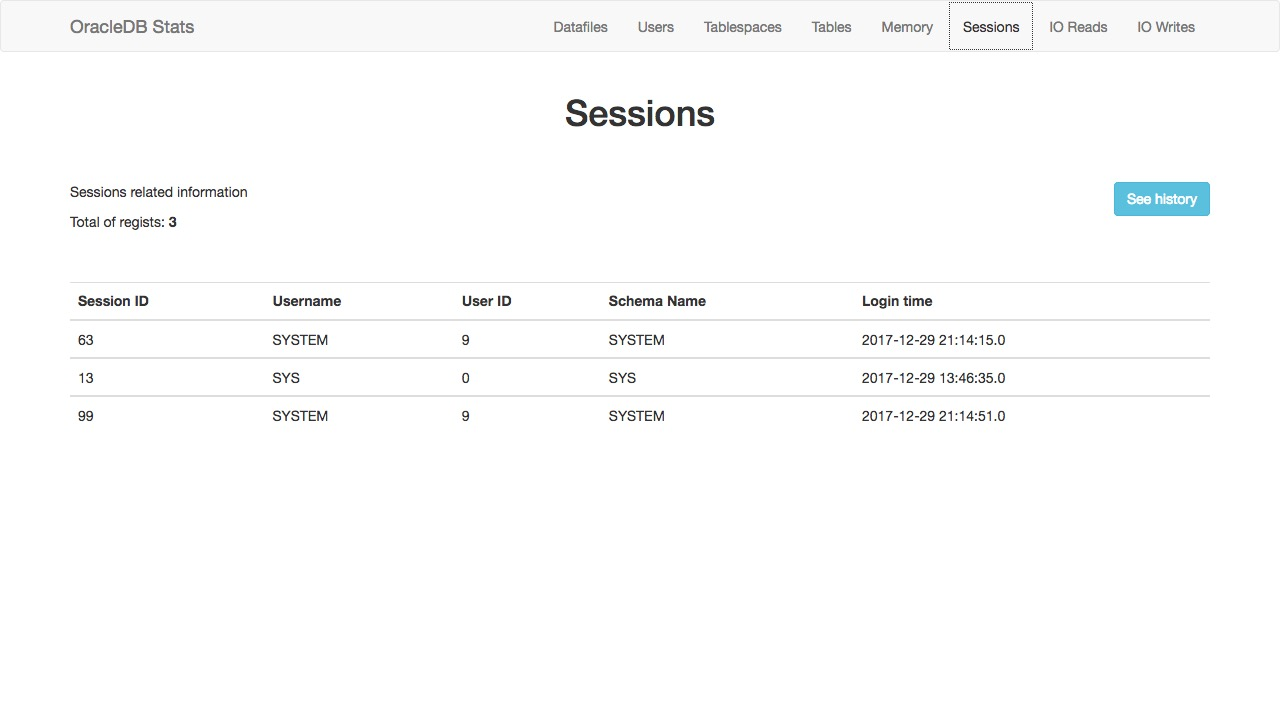
\includegraphics[width=\linewidth]{tex/img/sessions.jpg}
    \caption{Página correspondente às Sessions} 
    \label{fig:esquemarest}
\end{figure}
\newpage

\newpage
\section{Conclusão}\label{sec:Conclusion}

Os três sistemas de aprendizagem aqui explorados são diferentes entre eles. Enquanto que as Redes Neuronais Artificiais e a Aprendizagem por Reforço são utilizadas numa fase inicial de aprendizagem, os Algoritmos Genéticos são utilizados numa fase posterior na pesquisa por uma solução válida tendo em conta um contexto do momento.
Vemos muitas vezes sistemas em que se usa um conjunto de Redes Neuronais Artificiais com Algoritmos Genéticos para criar uma solução capaz de aprender e aplicar esse conhecimento noutros contextos.
As Redes Neuronais Artificiais assimilam-se ainda mais aos Algoritmos Genéticos na medida em que são ambos inspirados na biologia e nos sistemas biológicos. Já a Aprendizagem por Reforço é aplicado em situações em que o agente tem que interagir com o ambiente, aprendendo quais as ações que têm mais recompensas. Este tipo de comportamento é também similar ao que acontece na natureza.
Vemos assim que todos os sistemas tem origem na biologia e que apesar das suas diferenças relacionam-se de certo modo.
\newpage
\end{document}